
\documentclass[10pt,cn]{elegantbook}
\usepackage[utf8]{inputenc}
\usepackage[T1]{fontenc}
\usepackage{tgtermes}
\usepackage{amsmath}
\usepackage{amsfonts}
\usepackage{amssymb}
\usepackage{stmaryrd}
\usepackage{hyperref}
\hypersetup{colorlinks=true, linkcolor=blue, filecolor=magenta, urlcolor=cyan,}
\urlstyle{same}
\usepackage{graphicx}
\usepackage[export]{adjustbox}
\usepackage{mdframed}
\usepackage{booktabs,array,multirow}
\usepackage{esint}
\usepackage{xeCJK}
%\usepackage{adjustbox}
\usepackage[export]{adjustbox}
%\graphicspath{ {./images/} }

\usepackage{ulem}
\usepackage{hyperref}%目录跳转

\usepackage{fontspec} % 用于处理字体
%\setmainfont{TeX Gyre Termes} % 设置主要字体


%\usepackage{fancyhdr}   % 导入 fancyhdr 包,用于定制页眉和页脚
%\usepackage{datetime}   % 导入 datetime 包,用于格式化日期


\usepackage{graphicx}   % 导入 graphicx 包,以便插入图片


\usepackage{comment}

%\fancyhead[L]{20240722} % 左侧页眉
%\fancyhead[R]{\mydate\today} % 右侧页眉,显示当前日期,格式为“日 月 年”

\title{HappaMathsNotes}
\subtitle{数学笔记}
\author{OyamaHappa}
\date{\today}
\version{20240801092003}
\extrainfo{数学是人类智慧皇冠上最灿烂的明珠。——考特}
\logo{logo.jpg}
\cover{cover.jpg}



% 本文档命令
\usepackage{array}
\usepackage{mathdots}
\newcommand{\ccr}[1]{\makecell{{\color{#1}\rule{1cm}{1cm}}}}
% 修改目录深度
\setcounter{tocdepth}{3}

\everymath{\displaystyle}%用行间公式(displaystyle)的格式排版所有的行内公式


%\usepackage{verbatim}%在codeshow中已引用
\usepackage{tikz,tkz-euclide}
\usepackage{amsmath}
\usepackage{pgfplots}
%\usepackage{codeshow}%codeshow:为了在codeshow环境中,引用代码,并生成图形。

\usepackage{graphicx}
%\usepackage{subfigure}

\usepackage{breqn}%breqn 宏包主要提供了 dmath 和 dmath* 等几个环境,产生可以自动折行的显示公式。
\usepackage{longtable}%长表格,多页可以自动处理。

%【参与编译的文件列表。】
%\includeonly{preface,chapter01,chapter02,chapter03,chapter04,chapter05}%,%【参与编译的文件列表。】




\usepackage{amsmath}
\usepackage{amsfonts}
\usepackage{amssymb}
\usepackage{stmaryrd}
\usepackage{hyperref}
\hypersetup{colorlinks=true, linkcolor=blue, filecolor=magenta, urlcolor=cyan,}
\urlstyle{same}
\usepackage{graphicx}
\usepackage[export]{adjustbox}
\usepackage{mdframed}
\usepackage{booktabs,array,multirow}
\usepackage{esint}
\usepackage{xeCJK}
\usepackage{adjustbox}
\newcommand{\HRule}{\begin{center}\rule{0.5\linewidth}{0.2mm}\end{center}}
%\graphicspath{ {./images/} }
\usepackage{amsmath}
\usepackage{pifont}


\begin{document}
	
	\begin{titlepage}
		\begin{center}
			\vspace*{3cm}
			
			{\Large \textbf{HappaNotesBooks} }
			
			{\Large(试 用)}
			
			\vspace{1cm}
			
			{\Huge 数 \qquad 学}
			
			\vspace{0.5cm}
			
			OyamaHappa
			
			\vspace{1cm}
			
				{\Large 数列 }
			
			\vfill
			
			数学是人类智慧皇冠上最灿烂的明珠。——考特
			
		\end{center}
	\end{titlepage}
	
	%	\maketitle
	
	\tableofcontents
	%\listofchanges
	
	\mainmatter

	\chapter{数列}
	
	像上面的例子中,按一定次序排列的一列数叫做\textbf{数列}。数列中的每一个数都叫做这个数列的\textbf{项},如果数列 $\{a_n\}$ 的第 $n$ 项 $a_n$ 与 $n$
	之间的函数关系可以用一个公式来表示,这个公式就叫做这个数列的\textbf{通项公式}。项数有限的数列叫做\textbf{有穷数列},项数无限的数列叫做\textbf{无穷数列}。
	
	\section{等差数列}
	
	一般地,如果一个数列从第 $2$ 项起, 每一项与它的前一项的差等同一个常数,这个数列就叫做\textbf{等差数列},
	这个常数叫做等差数列的\textbf{公差}, 公差通常用字母 $d$ 表示。 
	
	\subsection{通项公式}
	
	等差数列 $\{a_n\}$ 的通项公式是
	\begin{center}
		\framebox{\begin{minipage}{12em}
				\begin{gather*}
					a_n = a_1 + (n - 1)d \text{。}
				\end{gather*}
		\end{minipage}}
	\end{center}
	
	如果在 $a$ 与 $b$ 中间插入一个数 $A$ ,使 $a$,$A$,$b$ 成等差数列,那么 $A$ 叫做 $a$ 与 $b$ 的 \textbf{等差中项}。
	
	如果 $A$ 是 $a$ 与 $b$ 的等差中项,那么 $A - a = b - A$,所以
	$$ A = \dfrac{a + b}{2} \text{。}$$
	
	\[a_{n+1}-a_{n}=d\]
%	$$a_{n}=a_{1}+(n-1)d$$
	
	等差数列 $\{a_n\}$ 的前 $n$ 项的和的公式
	\begin{center}
		\framebox{\begin{minipage}{12em}
				\begin{gather*}
					S_n = \dfrac{n(a_1 + a_n)}{2} \text{。}
				\end{gather*}
		\end{minipage}}
	\end{center}
	
	因为 $a_n = a_1 + (n - 1) d$,所以上面的公式又可写成
	\begin{center}
		\framebox{\begin{minipage}{12em}
				\begin{gather*}
					S_n = n a_1 + \dfrac{n(n - 1)}{2} d \text{。}
				\end{gather*}
		\end{minipage}}
	\end{center}
	
		\begin{center}
		\framebox{\begin{minipage}{20em}
				\begin{gather*}
						a_{n}=dn-d+a_{1} \Leftrightarrow \textbf{kn+b}
						\\
					    S_{n}=\dfrac{d}{2}n^{2}+(a_{1}-\dfrac{d}{2})n \Leftrightarrow \textbf{$ An^{2} +Bn$}
				\end{gather*}
		\end{minipage}}
	\end{center}
	
$$a_{n}=S_{n}-S_{n-1}$$

	\subsection{等差中项定理}
	
	$a_{n}+a_{n+2}=2a_{n+1}$
	$$a_{m}+a_{n}=a_{p}+a_{q} \Leftrightarrow \textbf{m+n=p+q}$$
	
	\subsection{前n项和的性质}
    
    \ding{172}
    
    $$S_{2n-1}=(2n-1)\cdot a_{n}$$
    $$S_{2n+1}=(2n+1)\cdot a_{n+1}$$
    $$S_{2n}=n\cdot (a_{n}+a_{n+1})$$
    
     \ding{173}
     
     $\dfrac{S_{2n+1}}{T_{2n+1}}=\dfrac{(2n+1)\cdot a_{n+1}}{(2n+1)\cdot b_{n+1}} = \dfrac{a_{n}}{b_{n}}$
     
     	\begin{center}
     	\framebox{\begin{minipage}{12em}
     			\begin{gather*}
     				\dfrac{S_{2n+1}}{T_{2n+1}} = \dfrac{a_{n}}{b_{n}}
     			\end{gather*}
     	\end{minipage}}
     \end{center}
     
      \ding{174}
      
      $ S_{n},S_{2n}-S_{n},S_{3n}-S_{2n}$构成等差数列,$d'=n^{2}d$
      
      \ding{175}
      
      $S_{n}=An^{2}+Bn$
      
      $\dfrac{S_{n}}{n}=An+B$
      
      $$\dfrac{S_{n}}{n}=\dfrac{d}{2}n+(a_{1}-\dfrac{d}{2}) \Rightarrow \text{公差为}\dfrac{d}{2}$$
      
      \section{等比数列}
      
      一般地,如果一个数列从第 $2$ 项起,每一项与它前一项的比等于同一个常数,
      这个数列就叫做\textbf{等比数列}, 这个常数叫做等比数列的\textbf{公比},
      公比通常用字母 $q$ 表示。
      
      等比数列 $\{a_n\}$ 的通项公式是
      \begin{center}
      	\framebox{\begin{minipage}{12em}
      			\begin{gather*}
      				a_n = a_1  q^{n - 1} \text{。}
      			\end{gather*}
      	\end{minipage}}
      \end{center}
      
      上面的公式还可以改写成
      $$ a_n = \dfrac{a_1}{q} q^n = c q^n \text{,}$$
      这里 $c = \dfrac{a_1}{q}$ ,它是一个不为零的常数。当 $q$ 是不等于 $1$ 的正数时,
      $y = q^x$ 是一个指数函数,而函数 $y = c q^x$ 是一个不为零的常数与指数函数的积。
      因此, 从图上看,表示数列 $\{c q^n\}$ 各项的点都在函数 $y = c q^x$ 的图像上。
      
      \subsection{递推公式}
      
      $$\dfrac{a_{n+1}}{a_{n}}=q \neq 0$$
      
       \subsection{通项公式}
       
       $$a_{n}=a_{1} \cdot q^{n-1} n \in N^{*}$$
       
        \subsection{等比中项定理}
        
        $a_{n} \cdot a_{n+2}=(a_{n+1})^{2}$
        
        $$a_{m}\cdot a_{n}= a_{s} \cdot a_{t} \leftrightarrow m+n=s+t$$
        
        $$\text{奇数项同号}$$
        $$\text{偶数项同号}$$
        
        \subsection{求和}
        
        $S_{n}=\dfrac{a_{1}\cdot (a-q^{n})}{1-q}=\dfrac{a_{1}}{1-q}-\dfrac{a_{1}}{1-q} \cdot q^{n}$
        $$S_{n}=\dfrac{a_{1}}{1-q}-\dfrac{a_{1}}{1-q} \cdot q^{n} \Leftrightarrow A-A\cdot q$$
        
        $a_{n}=a_{1}\cdot q^{n-1}$
        $$ =\dfrac{a_{1}-a_{n}\cdot q}{1-q}$$
        
        \subsection{性质}
        
        $S_{n},S_{2n}-S_{n},S_{3n}-S_{2n}$构成新等比数列且公比$q'=q^{n}$
        
        \section{数列求通项}
        
        \subsection{累加法}
        \subsubsection*{形式}
        $a_{n+1}=a_{n}+f(n)$
        \subsubsection*{例题}
        
        $a_{1}=2,a_{n+1}=a_{n}+\ln (1+\dfrac{1}{n})$
        
        \begin{tcolorbox}[colback=yellow!10!white, colframe=red!50!black]
        	$\ln (1+\dfrac{1}{n})=\ln \dfrac{n+1}{n} = \ln (n+1)-\ln n$
        	
            	$
            \left.
            \begin{aligned}
            a_{2}=a_{1}= \ln 2-\ln 1 \\
            a_{3}-a_{2}=\ln 3 -\ln 2\\
            ...\\
              a_{n}-a_{n-1}=\ln n-\ln (n-1)
            \end{aligned}
            \right\}
             \text{累加} \Rightarrow a_{n}-a_{1}=\ln n -\ln 1=\ln n
               $
               
                  
               $ \therefore$ $n \geq 2$时$a_{n}=2+\ln n$
               
               检验\quad n=1时,$a_{1}=2$
               
               $ \therefore $ $a_{n}=2+\ln n ,n \in N^{*}$
        \end{tcolorbox}
     
     
      \subsection{累乘法}
     \subsubsection*{形式}
     $a_{n+1}=a_{n} \cdot f(n)$
     \subsubsection*{例题}
     
     $a_{1}=1,a_{n+1}= \dfrac{n}{n+1} a_{n}$
     
     \begin{tcolorbox}[colback=yellow!10!white, colframe=red!50!black]
     	$\dfrac{a_{n+1}}{a_{n}}=\dfrac{n}{n+1}$
     	\\
     	$
     	\left.
     	\begin{aligned}
     		\dfrac{a_{2}}{a_{1}}= \dfrac{1}{2} \\
     		\dfrac{a_{3}}{a_{2}}= \dfrac{2}{3} \\
     		... \\
     		\dfrac{a_{n}}{a_{n-1}}= \dfrac{n-1}{n}
     	\end{aligned}
     	\right\}
     	\text{累乘} \Rightarrow \dfrac{a_{2}}{a_{1}} \cdot \dfrac{a_{3}}{a_{2}}...\dfrac{a_{n}}{a_{n-1}} = \dfrac{1}{2} \cdot \dfrac{2}{3} \cdot ... \dfrac{n-1}{n}
     	$
     	
     	
     	$ \therefore$ $n \geq 2$时$a_{n}=a_{1} \cdot \dfrac{1}{n} =\dfrac{1}{n}$
     	
     	检验\quad n=1时,$a_{1}=1$
     	
     	$ \therefore $ $a_{n}=\dfrac{1}{n} ,n \in N^{*}$
     \end{tcolorbox}
     
      \subsubsection{构造常数列}
      
      $(n+1)a_{n+1}=n a_{n}$
      
      令$b_{n}=n a_{n}$
      
      $\Rightarrow b_{n+1}=b_{n}$
      
      \{ $b_{n}$\} 为常数列,且$b_{n}=b_{1}=a_{1}=1$
      
      $ \therefore a_{n}=\dfrac{b_{n}}{n}=\dfrac{1}{n} \quad  n\in N^{*}$
      
         \subsection{构造法-待定系数法}
      \subsubsection*{形式}
      $a_{n+1}=p a_{n} + q$
      
       \subsubsection*{操作}
       
    \textbf{   构造等比}
    
    $a_{n+1}+ \lambda = p(a_{n}+ \lambda)  \Rightarrow \lambda =\dfrac{q}{p-1}$
    
\textit{    $\{a_{n}+\lambda \}$是公比为p,首项为$a_{1}+\lambda $的等比数列}

      \subsubsection*{例题}
      
      $a_{1}=1,a_{n+1}= 4 a_{n} +1$
      
      \begin{tcolorbox}[colback=yellow!10!white, colframe=red!50!black]
      
      令$a_{n+1}+k=4(a_{n}+k)$
      
      $3k=1 \Rightarrow k=\dfrac{1}{3}$
      
     $ \therefore \dfrac{a_{n+1}+\dfrac{1}{3}}{a_{n}+\dfrac{1}{3}}=4$
     
     $\Rightarrow \{a_{n}+\dfrac{1}{3}\}$ 是公比为4的等比数列
     
     $\therefore a_{n}+\dfrac{1}{3}=(a_{1}+\dfrac{1}{3}) \cdot 4^{n-1}=4^{n-1}$
     
     $\therefore a_{n}=4^{n-1}-\dfrac{1}{3} \quad n \in N^{*}$
      \end{tcolorbox}

     \subsection{构造法-同除以指数}
\subsubsection*{形式}
$a_{n+1}=p a_{n} + q^{n}$

\subsubsection*{操作}

\textit{两边同除$q^{n+1}$}

$\dfrac{a_{n+1}}{q^{n+1}}=\dfrac{p}{q}\cdot \dfrac{a_{n}}{q_{n}}$

转为待定系数法求解

\subsubsection*{例题}

$a_{1}=3,a_{n+1}= 3 a_{n} -3^{n}$

\begin{tcolorbox}[colback=yellow!10!white, colframe=red!50!black]
	
	$\dfrac{a_{n+1}}{3^{n+1}}=\dfrac{a_{n}}{3^{n}}-\dfrac{1}{3}$
	
	$\dfrac{a_{n+1}}{3^{n+1}}-\dfrac{a_{n}}{3^{n}}=-\dfrac{1}{3}$
	
	
\textit{	$\{\dfrac{a_{n}}{3^{n}}\}$ 是公差为$-\dfrac{1}{3}$的等差数列}
	
   $\dfrac{a_{n}}{3^{n}}=\dfrac{a_{1}}{3^{1}}+(n-1)(-\dfrac{1}{3})=-\dfrac{1}{3}n+\dfrac{4}{3}$
	
	$\therefore a_{n}=(4-n)3^{n-1} \quad n \in N^{*}$
\end{tcolorbox}

  \subsection{构造法-	取倒数}
\subsubsection*{形式}
$a_{n+1}=\dfrac{p a_{n}}{q a_{n+r}}$

\subsubsection*{操作}

\textit{两边同取倒数}

$\dfrac{1}{a_{n+1}}=\dfrac{q a_{n}+r}{p a_{n}}=\dfrac{r}{p}\dfrac{1}{a_{n}}+\dfrac{q}{p}$

转为待定系数法求解

\subsubsection*{例题}

$a_{1}=1,a_{n+1}= \dfrac{a_{n}}{1+a_{n}}$

\begin{tcolorbox}[colback=yellow!10!white, colframe=red!50!black]
	
	$\dfrac{1}{a_{n}+1}=\dfrac{1+a_{n}}{a_{n}}=\dfrac{1}{a_{n}+1}$
	
	$\dfrac{1}{a^{n+1}}-\dfrac{1}{a^{n}}=1$
	
	
	\textit{	$\{\dfrac{1}{a_{n}}\}$ 是公差为$1$的等差数列}
	
	$\dfrac{1}{a_{n}}=\dfrac{1}{a_{1}}+n-1=n$
	
	$\therefore a_{n}=\dfrac{1}{a_{n}}\quad n \in N^{*}$
\end{tcolorbox}

  \subsection{构造法-	取对数 }
\subsubsection*{形式}
$a_{n+1}=k {a_{n}}^{m}$

\subsubsection*{操作}

\textit{两边同取以k为底的对数}

$\uwave{{\log}_{k} a_{n+1}}={\log}_{k} (k{a_{n}}^{m})=1+m\uwave{ {\log}_{k} (k{a_{n}})}$

转为待定系数法求解

\section{列项相消}
分子=分母之差

\subsection*{\ding{172}}

$\dfrac{1}{n(n+1)}=\dfrac{n+1-n}{n(n+1)}=\dfrac{1}{n}-\dfrac{1}{n+1}$

\subsection*{\ding{173}}

$\dfrac{2}{n(n+1)}=2\cdot (\dfrac{1}{n}-\dfrac{1}{n+1})$

$\Rightarrow \dfrac{1}{n(n+2)}=\dfrac{n+2-n}{n(n+2)}\cdot \dfrac{1}{2}=\dfrac{1}{2}(\dfrac{1}{n}-\dfrac{1}{n+2})$

\subsection*{\ding{174}}

$\dfrac{1}{n(n+k)}=\dfrac{1}{k}\cdot \dfrac{n+k-n}{n(n+k)}=\dfrac{1}{k}(\dfrac{1}{n}-\dfrac{1}{n+k})$

\section{等差比数列}

等差$\times$等比

\subsection{错位相减}

$a_{n}=-\dfrac{2}{3^{n}},b_{n}=2n-1$

$c_{n}=-\dfrac{2b_{n}}{a_{n}}=(2n-1)\cdot 3^{n}$

$S_{n}?$

\subsubsection{\ding{172} 列}

$s_{n}=1\cdot 3^{1}+3\cdot 3^{2}+5\cdot3^{3}+...+(2n-3)\cdot 3^{n-1}+(2n-1)\cdot3^{n}$

\subsubsection{\ding{173} 乘}
$qS_{n}=1\cdot 3^{2}+3\cdot 3^{3}+...+(2n-3)\cdot 3^{n}+(2n-1)\cdot3^{n+1}$

\subsubsection{\ding{174} 减}

$-2S_{n}=1\cdot 3^{1}+2\cdot 3^{2}+2\cdot 3^{3}+... _2\cdot 3^{n}-(2n-1)\cdot 3^{n+1}$

\subsubsection{\ding{175} 除}

$=\dfrac{a_{1}(1-q^{n})}{1-q}=2\cdot \dfrac{3(1-3^{n})}{1-3}-3-(2n-1)\cdot 3^{n+1}=3^{n+1}-3-3-(2n-1)\cdot 3^{n+1}$

$-2S_{n}=-(2n-2)\cdot 3^{n+1}-6$

$S_{n}=(n-1)3^{n+1}+3$

\chapter{空间向量}


\begin{center}
	\adjustbox{max width=\textwidth}{
		\begin{tabular}{|c|c|c|}
			\hline
			\phantom{X} & 对称轴或对称中心、 对称平面 & 对称点坐标 \\
			\hline
			\multirow{7}{*}{\(P\left( {a,b,c}\right)\)} & \(x\) 轴 & \(\left( {a, - b, - c}\right)\) \\
			\cline{2-3}
			& \(y\) 轴 & \(\left( {-a,b, - c}\right)\) \\
			\cline{2-3}
			& \(z\) 轴 & \(\left( {-a, - b,c}\right)\) \\
			\cline{2-3}
			& \({Oxy}\) 平面 & \(\left( {a,b, - c}\right)\) \\
			\cline{2-3}
			& \({Oyz}\) 平面 & \(\left( {-a,b,c}\right)\) \\
			\cline{2-3}
			& \({Ozx}\) 平面 & \(\left( {a, - b,c}\right)\) \\
			\cline{2-3}
			& 坐标原点 & \(\left( {-a, - b, - c}\right)\) \\
			\hline
		\end{tabular}
	}
\end{center}

\section{点到直线的距离}

已知直线 \(l\) 的单位方向向量为 \(\mathbf{u}\) ,
\(A\) 是直线 \(l\) 上的定点, \(P\) 是直线 \(l\)
外一点,设 \(\overrightarrow{AP} = \mathbf{a}\) ,则向量 \(\overrightarrow{AP}\) 在
直线 \(l\) 上的投影向量 \(\overrightarrow{AQ} = \left( {\mathbf{a} \cdot \mathbf{u}}\right) \mathbf{u}\) . 在 Rt \(\bigtriangleup {APQ}\) 中,由
勾股定理,得 \({PQ} = \sqrt{{\left| \overrightarrow{AP}\right| }^{2} - {\left| \overrightarrow{AQ}\right| }^{2}} = \sqrt{{a}^{2} - {\left( a \cdot u\right) }^{2}}\) .

\begin{center}
	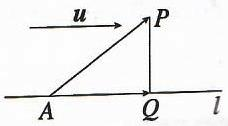
\includegraphics[max width=0.3\textwidth]{images/019111e7-c8b0-74a7-8b9e-0df758ddb65d_0_169880.jpg}
\end{center}



(1) 建立空间直角坐标系, 并求相应点的坐标.

(2) 求出直线的方向向量 \(\mathbf{a}\) 的坐标,并求 \(\left| \mathbf{a}\right|\) .

(3) 求以直线上某一特殊点为起点, 已知点为终

主的向量 \(\mathbf{b}\) 的坐标,并求 \(\left| \mathbf{b}\right|\) ,计算 \(\frac{\mathbf{a} \cdot \mathbf{b}}{\left| \mathbf{a}\right| }\) .

(4) 利用 \(\sqrt{{\left| \mathbf{b}\right| }^{2} - {\left( \frac{\mathbf{a} \cdot \mathbf{b}}{\left| \mathbf{a}\right| }\right) }^{2}}\) 求点到直线的距离.

\section{点到平面的距离}

已知平面 \(\alpha\) 的
法向量为 \(n,A\) 是平面 \(\alpha\) 内的定
点, \(P\) 是平面 \(\alpha\) 外一点. 过点 \(P\)
作平面 \(\alpha\) 的垂线 \(l\) ,交平面 \(\alpha\) 于
点 \(Q\) ,则点 \(P\) 到平面 \(\alpha\) 的距离 \({PQ} = \frac{\left| \overrightarrow{AP} \cdot n\right| }{\left| n\right| }\) .

\begin{center}
	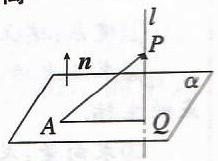
\includegraphics[max width=0.3\textwidth]{images/019111e7-c8b0-74a7-8b9e-0df758ddb65d_0_467128.jpg}
\end{center}
\end{document}
